%%
%% This is file `sample-sigconf-biblatex.tex',
%% generated with the docstrip utility.
%%
%% The original source files were:
%%
%% samples.dtx  (with options: `sigconf-biblatex')
%%
%% IMPORTANT NOTICE:
%%
%% For the copyright see the source file.
%%
%% Any modified versions of this file must be renamed
%% with new filenames distinct from sample-sigconf-biblatex.tex.
%%
%% For distribution of the original source see the terms
%% for copying and modification in the file samples.dtx.
%%
%% This generated file may be distributed as long as the
%% original source files, as listed above, are part of the
%% same distribution. (The sources need not necessarily be
%% in the same archive or directory.)
%%
%%
%% Commands for TeXCount
%TC:macro \cite [option:text,text]
%TC:macro \citep [option:text,text]
%TC:macro \citet [option:text,text]
%TC:envir table 0 1
%TC:envir table* 0 1
%TC:envir tabular [ignore] word
%TC:envir displaymath 0 word
%TC:envir math 0 word
%TC:envir comment 0 0
%%
%%
%% The first command in your LaTeX source must be the \documentclass
%% command.
%%
%% For submission and review of your manuscript please change the
%% command to \documentclass[manuscript, screen, review]{acmart}.
%%
%% When submitting camera ready or to TAPS, please change the command
%% to \documentclass[sigconf]{acmart} or whichever template is required
%% for your publication.
%%
%%
\documentclass[sigconf,natbib=false,nonacm,screen]{acmart}

% Automatic reference labels (\cref)
\usepackage[nameinlink]{cleveref}


% Semantic markup (analogously to \emph{})
\renewcommand\bold[1]{\textbf{#1}}
\newcommand\code[1]{%
	\texttt{#1}}
	%\textsf{#1}} % This looks more like Smalltalk
% TODO: apply existing italic emphasis
\newcommand\hardcode[1]{%
	\texttt{#1}}
\newcommand\name[1]{\textsc{#1}}
\newenvironment{multicode}{%
	\begin{quote}\sffamily\setlength{\parindent}{0pt}}{\end{quote}}


% SI units
\usepackage{siunitx}
% bold SI units
\sisetup{detect-all=true}


% Line-breaks after slashes
\newcommand\?{\hspace{0pt}}


% double-blinding
\makeatletter
\@ifclasswith{acmart}{anonymous}{%
	\newcommand{\ifanon}[2]{#1}%
}{%
	\newcommand{\ifanon}[2]{#2}%
}
\makeatother

\newcommand{\tdb}{\name{\ifanon{OurExistingOmniscientDebugger}{TraceDebugger}}}
\newcommand{\tfd}{\name{\ifanon{OurNewVisualizationTool}{trace\-4d}}}


% linebreaks in table cells
\usepackage{makecell}

% table notes below table (used for hacked footnotes)
\usepackage{threeparttable}

% yet another table package, don't allow for too much simplicity
\usepackage{tabularx}
\newcolumntype{L}{>{\raggedright\let\newline\\\arraybackslash\hspace{0pt}}X}
\newcolumntype{Y}{>{\centering\arraybackslash}X}
\usepackage{ragged2e}
\newcolumntype{M}[1]{>{\RaggedRight\hspace{0pt}}m{#1}}
\newcolumntype{B}[1]{>{\RaggedRight\hspace{0pt}}b{#1}}
\newcolumntype{P}[1]{>{\RaggedRight\hspace{0pt}}p{#1}}
\newcolumntype{C}[1]{>{\centering\let\newline\\\arraybackslash\hspace{0pt}}b{#1}}

% itemize-like item in table
% CREDITS: https://tex.stackexchange.com/a/150650/221054
\newcommand{\tabitem}{~~\llap{\textbullet}~~}


% tikz
\usepackage{tikz}
\usepackage{tikzscale}
\usetikzlibrary{calc}

% UML diagrams
\usepackage{pgf-umlcd}

% patch: UML self-associations
% based on CREDITS: https://tex.stackexchange.com/a/98023/221054
\newcommand{\selfCompositionSW}[3]{
	% 0.4: too high
	% 0.45: too low
	\draw[umlcd style,fill=\umldrawcolor,diamond-] (#1.south) -- ($(#1.south) - (0, 0.425)$);
	\draw[umlcd style] ($(#1.south) - (0, 0.425)$) -- ($(#1.west) - (0.75, 1)$);
	\draw[umlcd style] ($(#1.west) - (0.75, 1)$) -- ($(#1.west) - (0.75, 0)$);
	\draw[umlcd style,->] ($(#1.west) - (0.75, 0)$) -> (#1.west)
		node[midway, below]{#2}
		node[midway, above]{#3};
}
\newcommand{\selfCompositionEN}[3]{
	% 0.75: too left
	\draw[umlcd style,fill=\umldrawcolor,diamond-] (#1.east) -- ($(#1.east) + (0.25, 0)$);
	\draw[umlcd style] ($(#1.east) + (0.25, 0)$) -- ($(#1.north) + (0.8, 0.25)$);
	\draw[umlcd style] ($(#1.north) + (0.8, 0.25)$) -- ($(#1.north) + (0, 0.25)$);
	\draw[umlcd style,->] ($(#1.north) + (0, 0.25)$) -> (#1.north)
		node[midway, right]{#2}
		node[midway, left]{#3};
}


% \cites for natbib
% CREDITS: https://tex.stackexchange.com/a/537201/221054
\makeatletter
\newcommand{\citecomment}[2][]{\citenum{#2}#1\citevar}
\newcommand{\citeone}[1]{\citecomment{#1}}
\newcommand{\citetwo}[2][]{\citecomment[,~#1]{#2}}
\newcommand{\citevar}{\@ifnextchar\bgroup{;~\citeone}{\@ifnextchar[{;~\citetwo}{]}}}
\newcommand{\citefirst}{\@ifnextchar\bgroup{\citeone}{\@ifnextchar[{\citetwo}{]}}}
\newcommand{\cites}{[\citefirst}
\makeatother


% lowercase variants of \nameref
% CREDITS: https://tex.stackexchange.com/a/449775/221054
\usepackage{mfirstuc}[2017/11/14 v2.06 (NLCT)]

\makeatletter
\AtBeginDocument{%
	\newcommand\My@Macro[1]{#1}%
	\newcommand\My@Thirdoffive[5]{\My@Macro{#3}}%
	\renewcommand*\@namerefstar[1]{%
		\HyRef@StarSetRef{#1}\My@Thirdoffive
	}%
	\renewcommand*\T@nameref[1]{%
		\begingroup
		\let\label\@gobble
		\NR@setref{#1}\My@Thirdoffive{#1}%
		\endgroup
	}%
	\DeclareRobustCommand\fucnameref{%
		\@ifstar\fucnameref@star\fucnameref@nostar
	}%
	\newcommand\callemakefirstuc[1]{%
		\MakeLowercase{\emakefirstuc{#1}}%
	}%
	\newcommand\fucnameref@star[1]{%
		\begingroup
		\let\My@Macro=\callemakefirstuc
		\nameref*{#1}%
		\endgroup
	}%
	\newcommand\fucnameref@nostar[1]{%
		\begingroup
		\let\My@Macro=\callemakefirstuc
		\nameref{#1}%
		\endgroup
	}%
	\DeclareRobustCommand\ucnameref{%
		\@ifstar\ucnameref@star\ucnameref@nostar
	}%
	\newcommand\ucnameref@star[1]{%
		\begingroup
		\MFUhyphentrue
		\let\My@Macro=\ecapitalisefmtwords
		\nameref*{#1}%
		\endgroup
	}%
	\newcommand\ucnameref@nostar[1]{%
		\begingroup
		\MFUhyphentrue
		\let\My@Macro=\ecapitalisefmtwords
		\nameref{#1}%
		\endgroup
	}%
	\DeclareRobustCommand\lcnameref{%
		\@ifstar\lcnameref@star\lcnameref@nostar
	}%
	\newcommand\lcnameref@star[1]{%
		\begingroup
		\let\My@Macro=\MakeLowercase
		\nameref*{#1}%
		\endgroup
	}%
	\newcommand\lcnameref@nostar[1]{%
		\begingroup
		\let\My@Macro=\MakeLowercase
		\nameref{#1}%
		\endgroup
	}%
}%
\makeatother


%%
%% \BibTeX command to typeset BibTeX logo in the docs
\AtBeginDocument{%
	\providecommand\BibTeX{{%
	Bib\TeX}}}

%% Rights management information.  This information is sent to you
%% when you complete the rights form.  These commands have SAMPLE
%% values in them; it is your responsibility as an author to replace
%% the commands and values with those provided to you when you
%% complete the rights form.
%\setcopyright{acmcopyright}
%\copyrightyear{2018}
%\acmYear{2018}
%\acmDOI{XXXXXXX.XXXXXXX}


\setcopyright{none}

\settopmatter{printacmref=false} % Removes citation information below abstract
\renewcommand\footnotetextcopyrightpermission[1]{} % removes footnote with conference information in first column


%%
%% Submission ID.
%% Use this when submitting an article to a sponsored event. You'll
%% receive a unique submission ID from the organizers
%% of the event, and this ID should be used as the parameter to this command.
%%\acmSubmissionID{123-A56-BU3}

%%
%% For managing citations, it is recommended to use bibliography
%% files in BibTeX format.
%%
%% You can then either use BibTeX with the ACM-Reference-Format style,
%% or BibLaTeX with the acmnumeric or acmauthoryear sytles, that include
%% support for advanced citation of software artefact from the
%% biblatex-software package, also separately available on CTAN.
%%
%% Look at the sample-*-biblatex.tex files for templates showcasing
%% the biblatex styles.
%%


%%
%% The majority of ACM publications use numbered citations and
%% references, obtained by selecting the acmnumeric BibLaTeX style.
%% The acmauthoryear BibLaTeX style switches to the "author year" style.
%%
%% If you are preparing content for an event
%% sponsored by ACM SIGGRAPH, you must use the acmauthoryear style of
%% citations and references.
%%
%% Bibliography style
\RequirePackage[
	datamodel=acmdatamodel,
	style=acmnumeric,
	]{biblatex}

%% Declare bibliography sources (one \addbibresource command per source)
\addbibresource{paper.bib}

%%
%% end of the preamble, start of the body of the document source.
\begin{document}

%%
%% The "title" command has an optional parameter,
%% allowing the author to define a "short title" to be used in page headers.
% TODO: Discuss title
\title{Bringing Objects to Life: Supporting Program Comprehension through Animated 2.5D Object Maps from Program Traces}

%%
%% The "author" command and its associated commands are used to define
%% the authors and their affiliations.
%% Of note is the shared affiliation of the first two authors, and the
%% "authornote" and "authornotemark" commands
%% used to denote shared contribution to the research.
\author{Christoph Thiede}
\email{christoph.thiede@student.hpi.de}
\orcid{0000-0002-7442-8216}
\affiliation{%
	\institution{Hasso Plattner Institute}
	\city{University of Potsdam}
	\country{Germany}
}

%%
%% By default, the full list of authors will be used in the page
%% headers. Often, this list is too long, and will overlap
%% other information printed in the page headers. This command allows
%% the author to define a more concise list
%% of authors' names for this purpose.
%\renewcommand{\shortauthors}{Thiede et al.}

%%
%% The abstract is a short summary of the work to be presented in the
%% article.
% !TeX root = ../paper.tex
\begin{abstract}
	Program comprehension is a key activity in software development.
	Several visualization approaches such as software maps have been proposed to support programmers in exploring the architecture of software systems, while little attention has been paid to the exploration of program behavior and programmers still rely on traditional code browsing and debugging tools to build a mental model of a system's behavior that connects abstract concepts to implementation artifacts.
	We propose a novel approach to visualizing program behavior through \emph{animated 2.5D object maps} that depict particular objects and their interactions from a program trace.
	We describe our implementation of this approach and evaluate it for different program traces through an experience report and performance measurements.
	Our results indicate that our approach can be beneficial for program comprehension tasks, but that further research is needed to improve scalability and usability.
\end{abstract}


%%
%% The code below is generated by the tool at http://dl.acm.org/ccs.cfm.
%% Please copy and paste the code instead of the example below.
%%
% TODO: Discuss CCS concepts later
\begin{CCSXML}
<ccs2012>
	<concept>
		<concept_id>10003120.10003145.10003146</concept_id>
		<concept_desc>Human-centered computing~Visualization techniques</concept_desc>
		<concept_significance>500</concept_significance>
	</concept>
	<concept>
		<concept_id>10011007.10011006.10011073</concept_id>
		<concept_desc>Software and its engineering~Software maintenance tools</concept_desc>
		<concept_significance>100</concept_significance>
	</concept>
</ccs2012>
\end{CCSXML}

\ccsdesc[500]{Human-centered computing~Visualization techniques}
\ccsdesc[100]{Software and its engineering~Software maintenance tools}

%%
%% Keywords. The author(s) should pick words that accurately describe
%% the work being presented. Separate the keywords with commas.
% TODO: Discuss keywords later
\keywords{software visualization, software maps, object-oriented programming, program comprehension, omniscient debugging}

% TODO: Fill in ACM Reference Format later
%\received{20 February 2007}
%\received[revised]{12 March 2009}
%\received[accepted]{5 June 2009}

%% A "teaser" image appears between the author and affiliation
%% information and the body of the document, and typically spans the
%% page.
\begin{teaserfigure}
	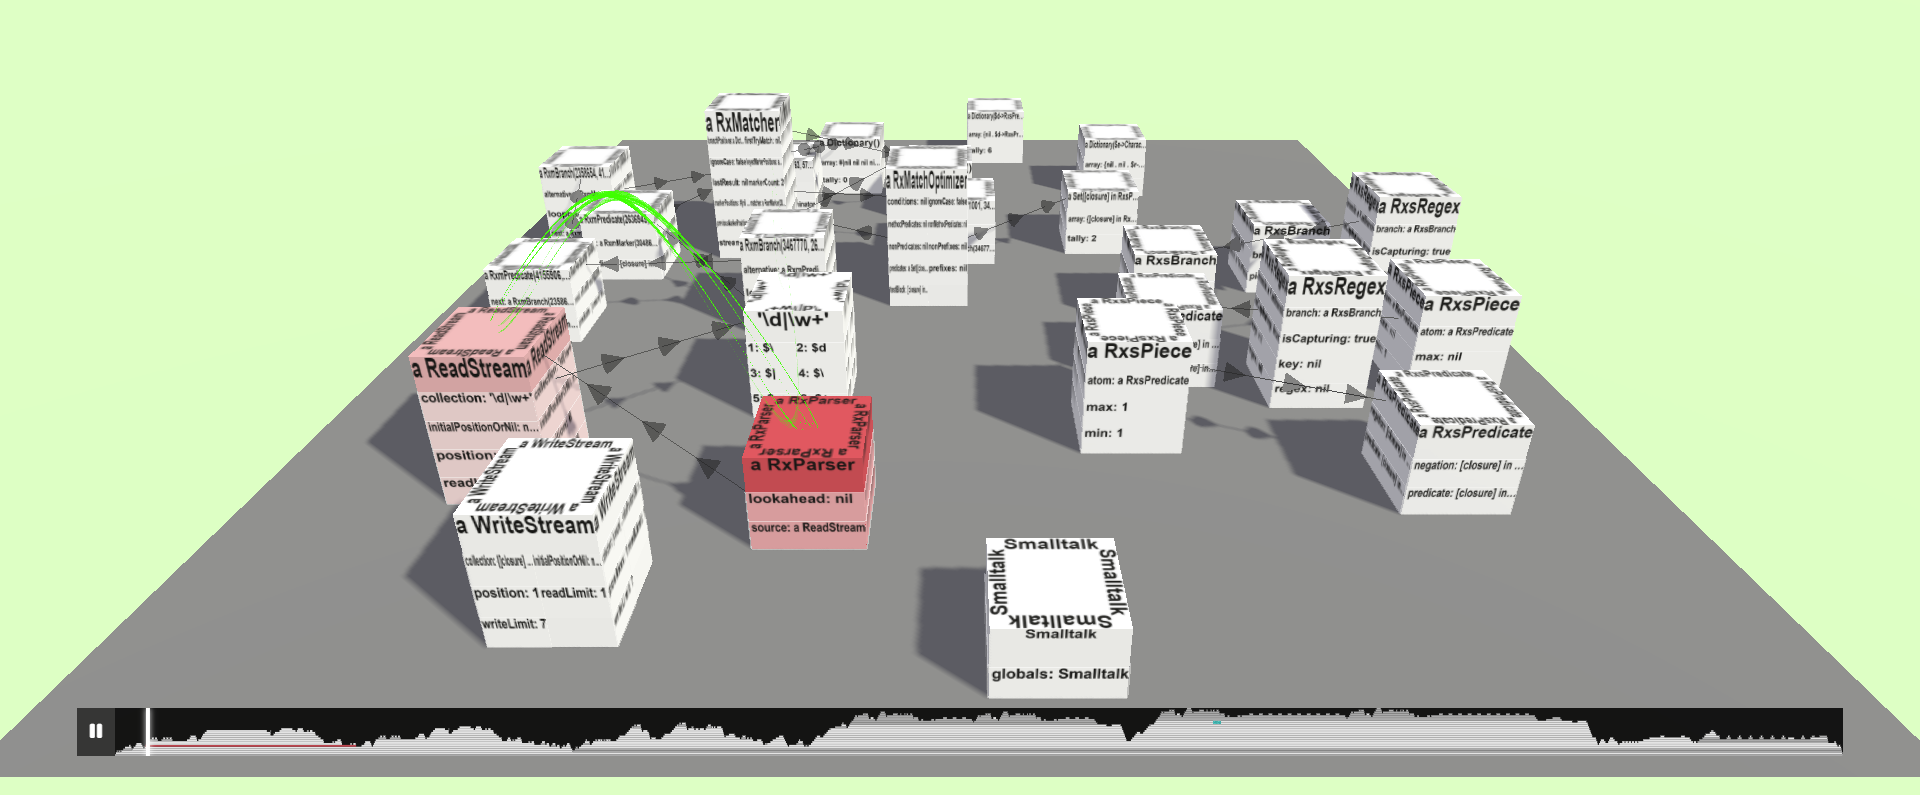
\includegraphics[width=\textwidth]{trace4d}
	\caption{
		Screenshot of an animated object map displaying a program trace for the construction of a regular expression matcher in the Squeak/Smalltalk programming environment.
		Blocks represent objects, arrows display references between objects, and color highlights and trails show object activations.
		The timeline at the bottom provides a temporal overview of the program trace and allows users to control the animation.
	}
	\Description{TODO}
	\label{fig:teaser}
\end{teaserfigure}
% TODO: Zoom in more?

%%
%% This command processes the author and affiliation and title
%% information and builds the first part of the formatted document.
\maketitle

% !TeX root = ../paper.tex
\section{Introduction}
\label{sec:introduction}

Exploring and understanding software systems play a central role in software development.
Programmers frequently get thrown into unknown systems that they want to fix, change, or extend.
For this, they need to build up a mental model that connects the system's visible behavior to its high-level architecture and low-level implementation artifacts.
%Research has shown that programmers spend 58\% of their time understanding code bases~\cite{xia2017measuring}.

Traditionally, programmers explore software systems by reading their source code.
An alternative approach is to explore the system's behavior by example:
programmers can start by invoking the system with a particular input or by running a test case and then use a debugger to step through the program's execution, identify relevant units and actors, and explore their interactions.
As traditional debuggers are constrained to the temporal execution order of the program, \emph{omniscient debuggers} (also referred to as \emph{time-travel debuggers} or \emph{back-in-time debuggers}) exist that record a \emph{program trace} and allow programmers to explore the program's behavior in a non-linear fashion~\cite{lewis2003debugging,hofer2006design,pothier2009back,lienhard2008practical,thiede2023object}.
However, omniscient debuggers are not well suited for exploring large program traces involving several subsystems and dozens of interacting objects:
while their fine-grained display of source code and variables is useful for debugging-related activities, it impedes the exploration of the system's high-level architecture and behavior.

On the other hand, several visualization approaches have been proposed to support programmers in exploring the architecture of software systems.
In particular, \emph{software maps} that display the static structure of systems using several metaphors such as cities or forests were found to be useful for program comprehension tasks~\cite{wettel2007visualizing,atzberger2021softwareforest,limberger2022visual}.
Yet, most approaches neglect the dynamic behavior of systems and take a coarse-grained view of their structure, which makes them unsuitable for developing a mental model of the system's behavior that situates particular interacting objects and connects them to the overall functioning of the system.

To bridge this gap between coarse-grained static software maps and fine-grained omniscient debugging views, we propose a novel approach for visualizing the behavior of object-oriented software systems through animated 2.5D maps depicting particular objects and their interactions from a program trace.
In particular, we make the following contributions:

\begin{enumerate}
	\item We present a novel visualization approach for ob\-ject-ori\-ent\-ed program behavior through animated 2.5D object maps.
	\item We describe the implementation of our prototype \tfd{} that applies this approach using program traces from a Squeak/\?Smalltalk environment and the THREE.js 3D library.
	\item We discuss the potential and limitations of our approach by reporting on our experience with it and by evaluating the performance of our implementation for different program traces.
\end{enumerate}

We make all artifacts of this work available at a public repository\footnote{\ifanon{\url{https://github.com/user/repo} (blinded)}{\url{https://github.com/LinqLover/trace4d}}}.

The remainder of this paper is structured as follows:
in \cref{sec:related_work}, we discuss related work on software maps, object-oriented programs, and program traces.
In \cref{sec:visualization_approach}, we present our visualization approach for program traces.
In \cref{sec:implementation}, we describe our implementation of this approach.
In \cref{sec:use_case}, we describe the use of our visualization tool by an example.
In \cref{sec:discussion}, we discuss the potential and limitations of 2.5D object maps through an experience report and a performance evaluation.
Finally, we conclude and discuss future work in \cref{sec:conclusion}.

% !TeX root = ../paper.tex
\section{Related Work}
\label{sec:related_work}

% !TeX root = ../paper.tex
\section{Visualization Approach}
\label{sec:visualization_approach}

To support the comprehension of object-oriented programs, we propose \emph{animated 2.5D object maps} as a novel visualization approach for program traces.
In the following, we describe the prerequisites and the design of our approach.

\subsection{Data Model}
\label{sec:visualization_approach/data_model}

\begin{figure}
	\includegraphics[width=\linewidth]{sections/03_visualization_approach/data_model.tikz}
	\caption{UML class diagram showing the data model of an object-oriented program trace for the visualization.}
	\Description{TODO}
	\label{fig:visualization_approach/data_model}
\end{figure}

%For the data source of the visualization, we assume a simple program trace model for object-oriented programs~(\cref{fig:visualization_approach/data_model}).
The data source of our visualization is the program trace of an object-oriented program.
%An object is characterized by its \emph{identity} which distinguishes it from all other objects in the system, its \emph{state} which is represented by its fields such as array elements and instance variables, and its \emph{behavior} which is described by methods that implement the reception of messages~\cite{thiede2023time}.
In this programming paradigm, all behavior is described as \emph{messages} sent from one object to another.
Each object is characterized by its \emph{identity} which distinguishes it from all other objects in the system, its \emph{state} which is represented by its fields such as array elements and instance variables, and its \emph{behavior} which is implemented by methods that are invoked to receive messages~\cite{thiede2023time}.

We assume a minimal data model of the program trace~(\cref{fig:visualization_approach/data_model}):
the \emph{call tree} is represented as a composite structure of \emph{stack frames} each of which specifies a time interval, an invoked method, and a receiver object.
Each \emph{object} is assigned a label, a list of named fields, and a class.
%The value of each \emph{field} can be a reference to another object or a flat string representation.
Each \emph{class} is described through a name and an organizational path in the file or package structure of the software system.
We neglect runtime changes to the state, label, or class membership of objects as well as metaprogramming specifics such as the implementation of classes or methods as objects.
% TODO: we also neglect coroutine, multiple processes, etc. but is this the right place to mention all of that?

\subsection{Visual Mapping}
\label{sec:visualization_approach/mapping}

We describe the design of our visualization and the mapping of parts from the program trace to elements and visual variables of our visualization~(\cref{fig:teaser}).
At the highest level, an animated 2.5 object map is an interactive information landscape that displays objects and their interactions from the program trace.
Users can replay the program trace and watch the \emph{activation} of objects, i.e., the execution of any of their methods, and the their \emph{interaction}, i.e., the exchange of messages between two objects.
They can unrestrictedly navigate through the visual scene using their keyboard and pointing devices and view the map from all sides.

\paragraph{Objects}
\label{sec:visualization_approach/mapping/objects}

\begin{figure}
	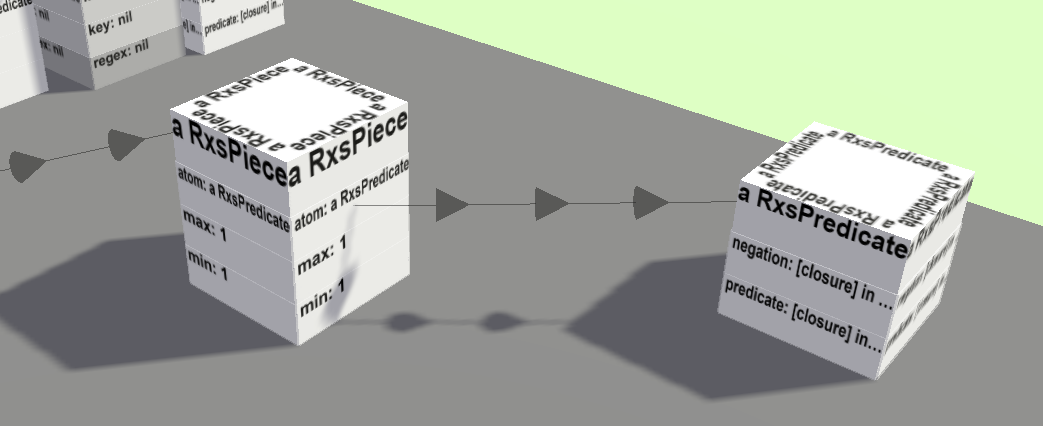
\includegraphics[width=\linewidth]{sections/03_visualization_approach/mapping/objects}
	\caption{Visual mapping of objects, fields, and references to block entities, plates, and arrows in the object map.}
	\Description{TODO}
	\label{fig:visualization_approach/mapping/objects}
\end{figure}

Each object is represented as a square cuboid \emph{block} entity that displays the label and fields of the object~(\cref{fig:visualization_approach/mapping/objects}).
To maximize legibility from any perspective, the label is repeated on all four sides and in four orientations on the top of the block.
Fields are displayed as \emph{plates} that are arranged in a row-wise uniform-sized grid layout and repeated on each side of the block for better legibility.
References between objects are rendered as \emph{directed arrows} from the closest plate of the referencing field to the closest label of the referenced object's entity.
To indicate the direction of arrows, we place between one and ten evenly distributed \emph{chevrons} on the arrow line; each chevron is displayed as a cone whose direction can be recognized from any perspective.

\paragraph{Object graph}
\label{sec:visualization_approach/mapping/object_graph}

All object blocks are placed on a plane in the 2.5D object map.
For their arrangement, we define a force-directed graph layout~\cite{fruchterman1991graph}.
Between each pair of object blocks $a$ and $b$, we apply several \emph{weighted attractive forces} based on the class membership ($F_\text{class}$), the organizational proximity of classes ($F_\text{org}$), and the references ($F_\text{ref}$) and communication ($F_\text{comm}$) between objects.
In the following definitions, the respective $w$ denote the weight of each force and $\text{org}(o)$ denotes the organizational path of an object $o$'s class (e.g., a file path):

%\begin{equation}
%	\begin{split}
%		F_{\text{class}}(a, b) &= w_{\text{class}}\left(\begin{cases}1, & \text{if $\text{class}(a) = \text{class}(b)$;} \\ 0, & \text{otherwise}.\end{cases}\right) \,, \\
%		F_{\text{org}}(a, b) &= w_{\text{org}}\bigl(\text{LCP}\footnotemark\bigl(\text{org}\footnotemark(a), \text{org}(b)\bigr)\bigr) \,, \\
%		F_{\text{ref}}(a, b) &= w_{\text{ref}}\left(\left|\bigl\{ (k, v) \in \text{fields}(a) ~\middle\vert~ v = b \bigr\}\right|\right) \,, \\
%		F_{\text{comm}}(a, b) &= w_{\text{comm}}\big(\big|\big\{\text{frame }f ~\big\vert \\
%			& \hphantom{= w} \text{$f$.receiver} = a \wedge \text{$f$.parent.receiver} = b\big\}\big|\big) \, .
%	\end{split}
%\end{equation}
%\addtocounter{footnote}{-1}
%\footnotetext{$\text{LCP}(u, v)$: Largest common prefix of two sequences $u$ and $v$.}
%\footnotetext{$\text{org}(o)$: Organizational path to an object $o$'s class (e.g., a file path).}

\begin{algorithm}
	$F_{\text{class}}(a, b) = \begin{cases}w_{\text{class}}, & \text{if $\text{class}(a) = \text{class}(b)$;} \\ 0, & \text{otherwise}.\end{cases}$ \;
	$F_{\text{org}}(a, b) = w_{\text{org}}\bigl(\text{commonPrefixLength}(\text{org}(a), \text{org}(b))\bigr)$ \;
	$F_{\text{ref}}(a, b) = w_{\text{ref}}\bigl(\text{number of fields in $a$ that reference $b$}\bigr)$ \;
	$F_{\text{comm}}(a, b) = w_{\text{comm}}\bigl(\text{number of messages from $a$ to $b$}\bigr)$ \;
\end{algorithm}

\begin{table}
	\centering
	\caption{
		Default configuration of force weights for the object graph layout (columns represent assignments).
		References between objects dominate the layout while organizational proximity and communication between objects are weighted lower.
		Users can override these weights for specific program traces.
	}
	\label{tab:visualization_approach/mapping/object_graph/default_configuration}
	\begin{threeparttable}
		\centering
		{\footnotesize
		% !TeX root = ../../../../paper.tex
{\setlength\tabcolsep{3pt}
\begin{tabular}{cccc c cc}
	\toprule

	\multicolumn{1}{c}{\bold{$w_{\text{class}}$}}	&
	\multicolumn{1}{c}{\bold{$w_{\text{org}}$}}	&
	\multicolumn{1}{c}{\bold{$w_{\text{ref}}$}}	&
	\multicolumn{1}{c}{\bold{$w_{\text{comm}}$}}	&
		&
	\multicolumn{1}{c}{\bold{$w_{\text{repulse}}$}}	&
	\multicolumn{1}{c}{\bold{$w_{\text{center}}$}}	\\

	\midrule

	$0.001$	&
	$F \mapsto 0.005 \left(\log_{10}(F) + 1\right)$	&
	$0.1$	&
	$0.00001$	&
		&
	$0.2$	&
	$0.00142$	\\

	\bottomrule
\end{tabular}}
}
	\end{threeparttable}
\end{table}

In addition to the attractive forces, we define globally weighted \emph{repulsion} and \emph{centripetation} forces on all blocks to control the entropy of the graph, and we define \emph{radial constraints} to avoid collisions between blocks.

We provide an empirical base configuration for all force weights but enable users to override them for specific program traces.
By default, we weight reference forces the highest and organizational forces the lowest with a distance of six orders of magnitudes and scale organizational forces logarithmically~(\cref{tab:visualization_approach/mapping/object_graph/default_configuration}).
This configuration fosters a state-centric layout of the object graph while leaving a margin for the characteristic of particular program traces (e.g., their ratio between intrinsic and extrinsic state~\cite[p. 218ff]{gamma1994design}) towards a more dataflow-driven layout.
Additionally, users can drag and drop blocks to customize the layout.
To reduce response times~\cite[chap. 11]{shneiderman2005designing} and maintain an experience of immediacy~\cite{ungar1997debugging}, we render the graph in regular update intervals before the force simulation has converged.

\paragraph{Object selection}
\label{sec:visualization_approach/mapping/object_selection}

Usually, even after restricting the object graph to the receivers from the call tree~(\cref{sec:visualization_approach/data_model}), only a small part of it is relevant for comprehending the high-level behavior of a program while many other objects fulfill lower-level implementation details.
In our visualization, we use a filtering system for excluding objects based on their label, class, or organization.
Similarly to the layout configuration~(\lcnameref{sec:visualization_approach/mapping/object_graph}), we provide an empirical default configuration that excludes certain base objects such as collections, booleans, and numbers, but allow users to customize these filters.

\paragraph{Object behavior}
\label{sec:visualization_approach/mapping/object_behavior}

The color of each object block displays its recent activity:
\emph{inactive} blocks are colored in a neutral light gray while \emph{active} blocks whose objects have received a message recently are highlighted in a bright red~(\cref{fig:visualization_approach/mapping/object_behavior}).
After the control flow passes on to other objects, blocks linearly fade back to the base color within one second, thus applying a single-hue continuous sequential color scheme by Brewer et al.\footnote{Cynthia Brewer and Mark Harrower. 2013 -- 2021. ColorBrewer: Color Advice for Cartography. Pennsylvania State University. \textsc{URL}: \url{https://colorbrewer2.org/}}

\begin{figure}
	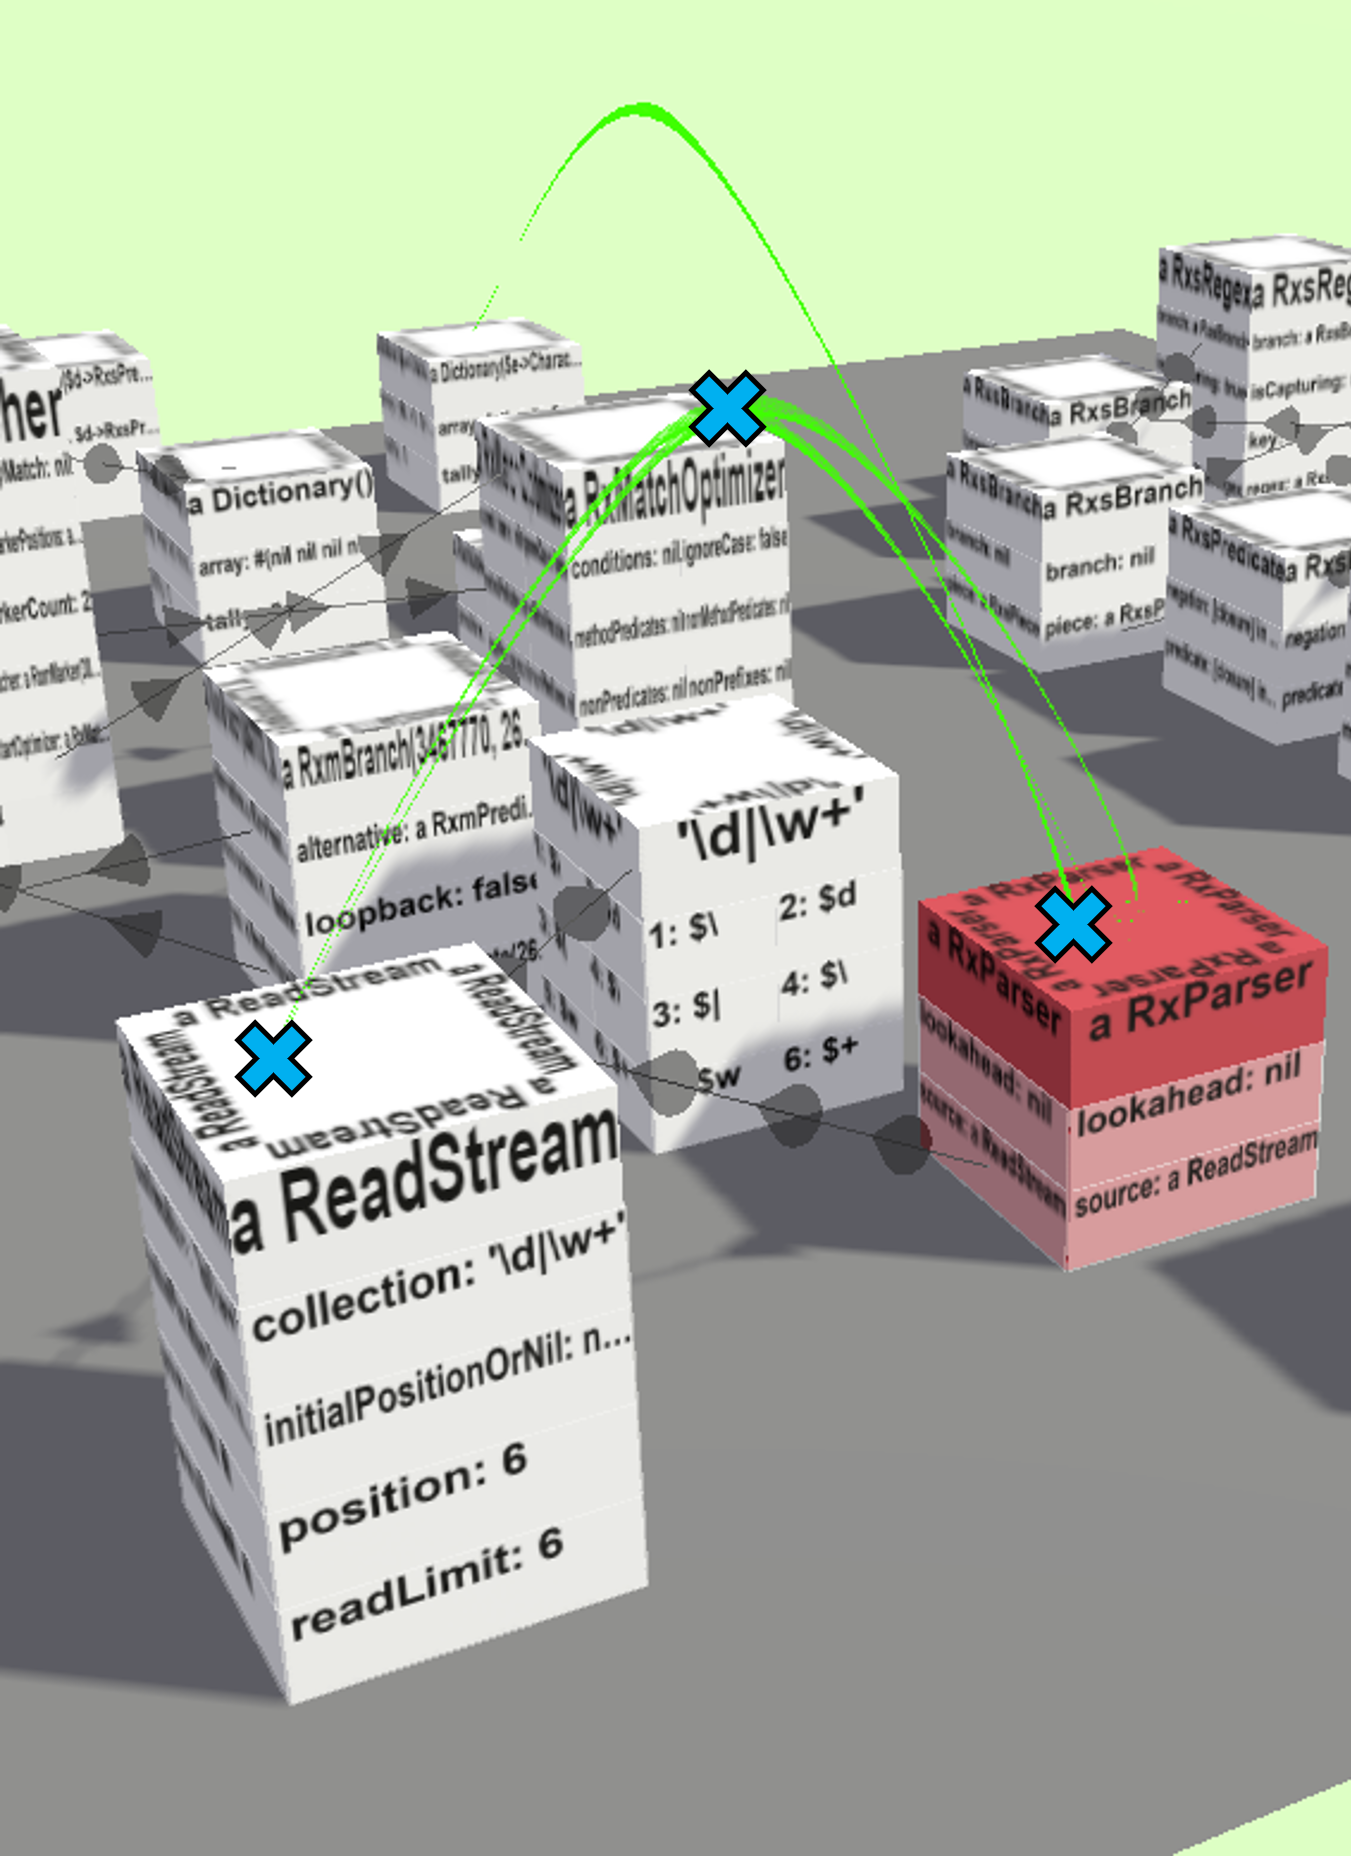
\includegraphics[width=\linewidth]{sections/03_visualization_approach/mapping/object_behavior}
	\caption{
		Visual mapping of object behavior to color and trail in the object map.
		The intensity of the red color indicates the recency of the last message received by each object.
		The gradient trail connects the most recent object activations (control points of the curve are marked with a \protect\texticon{sections/03_visualization_approach/mapping/object_behavior_cross} cross).
	}
	\Description{TODO}
	\label{fig:visualization_approach/mapping/object_behavior}
\end{figure}

Next to the color coding, a \emph{trail} connects the $k = 15$ most recent object activations to support the delayed observation of short activations and the recognition of exact activation order.
The trail curve is based on a centripetal Catmull-Rom spline~\cite{catmull1974class} whose control points are placed on the top of each relevant block and are alternated with intermediate points between blocks.
Block control points are normally randomized to make multiple activations of the same object distinguishable.
Intermediate control points are vertically elevated to give the curve a wave-like shape that makes activated objects identifiable.
The direction of the trail is displayed by continuously moving it to the next object during the animation and applying a linear translucency gradient to fade out the tail of the curve.

\paragraph{Timeline}
\label{sec:visualization_approach/mapping/timeline}

The object map integrates a \emph{timeline} overlay at the bottom of the viewport that provides a time-centric navigational aid.
The timeline consists of two widgets stacked on top of each other~(\cref{fig:visualization_approach/mapping/timeline}):
a \emph{player} with a slider and a play/pause button indicates the current point in time of the program trace and allows to control the time and animation state.
Behind the player, a collapsed \emph{flame graph} displays the course of the call stack depth.
Users can resize the timeline to explore the full call tree hierarchy and examine single frames in the flame graph.

Both the flame graph and the object map are interactively connected, i.e., users can hover an object in the map to discover all of its activations in the timeline, or vice versa, they can click on a frame to forward or rewind the trail in the map to the relevant object activation.
Thus, object map and timeline provide two orthogonal means for navigating through the object-oriented program trace with different granularities.

\begin{figure}
	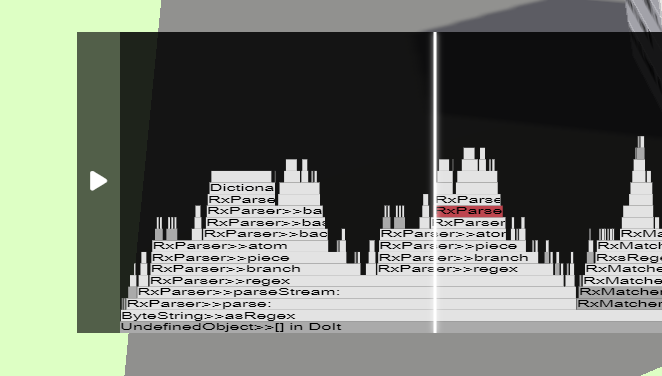
\includegraphics[width=\linewidth]{sections/03_visualization_approach/mapping/timeline}
	\caption{
		Timeline overlay with widgets for controlling the playback of the program trace and a flame graph with a variable degree of detail for navigating the call tree.
		The flame graph and the object map are interactively connected, e.g., the user can hover a frame to highlight the corresponding object in the map.
	}
	\Description{TODO}
	\label{fig:visualization_approach/mapping/timeline}
\end{figure}

% !TeX root = ../paper.tex
\section{Implementation}
\label{sec:implementation}

Here we describe the implementation of animated 2.5D object maps in our prototype \tfd{} that displays program traces from a Squeak/Smalltalk environment in a web application.

\paragraph{Program tracing}
\label{sec:implementation/program_tracing}

Squeak/Smalltalk is an interactive programming environment that is based on the object-oriented paradigm (everything is an object, including classes, methods, and stack frames) and offers programmers rich control for inspecting and manipulating all parts of the system (by instrumenting method objects, recording stack frame objects, etc.)~\cite{ingalls1997back,rowledge2001tour,thiede2023squeak}.
We use the \tdb{}\footnote{\ifanon{\url{https://github.com/user/repo} (blinded)}{\url{https://github.com/hpi-swa-lab/squeak-tracedebugger}}}\ifanon{}{~\cite{thiede2023object}}, which is an omniscient debugger for Squeak, to record a program trace of interesting behavior such as compiling a method, matching a string against a regular expression, or handling user events in a graphical user interface (GUI).

We serialize the resulting program trace consisting of a call tree, an object graph, and a class hierarchy and export it to a JSON file.
To retrieve the fields for each object, we use Squeak's built-in inspector tool~\cite[chap. 6, sec. 3]{thiede2023squeak} which collects all instance variables or array elements from each object but also provides higher-level views on the state of known domain objects; for instance, a dictionary will not be presented with its internal overallocation array structure but with a more comprehensible collection of key-value pairs.
Regarding the objects referenced as values from fields, we only include those objects in the serialization that receive at least one message in the program trace but only store a flat string representation of any other objects to avoid traversing the entire object graph of the system whose largest part is not relevant to the particular program trace.

\paragraph{Visualization}
\label{sec:implementation/visualization}

We implement the visualization frontend of \tfd{} as a JavaScript web application.
The web app retrieves a serialized program trace and offers a programmatical interface for customizing the visual configuration~(\cref{sec:visualization_approach/mapping/object_graph,sec:visualization_approach/mapping/object_selection}).
To build the 2.5D object map, we generate and display a 3D scene from the program trace using the JavaScript 3D library \name{three.js}\footnote{\url{https://threejs.org/}} and layout the object blocks using the \hardcode{d3-force} module of the visualization framework \name{d3.js}\footnote{\url{https://d3js.org/}}.
To build the timeline, we create a flame graph using the \hardcode{d3-flame-graph} plugin for \name{d3.js}\footnote{\url{https://github.com/spiermar/d3-flame-graph}} and combine it with a custom HTML widget for the player controls%
\footnote{As \hardcode{d3-flame-graph} at the time of writing does not support a notion of starting points but only lengths for frames, we inject auxiliary transparent frames into the flame graph to adjust the horizontal layout of actual frames (see \ifanon{\url{https://gist.github.com/user/id} (blinded)}{\url{https://github.com/spiermar/d3-flame-graph/issues/227}}).}%
.
To animate the visualization, we traverse the call tree with a configurable speed (defaulting to 50 bytecode instructions per second) and update the color highlights and trail for activated objects at each animation tick.

% !TeX root = ../paper.tex
\section{Use Case: Exploring Internals of a Regular Expression Engine}
\label{sec:use_case}

To illustrate how animated object maps can support program comprehension, we describe how a fictive programmer can use the \tfd{} visualization to explore the way a regular expression engine constructs a matcher from a pattern.
The \code{Regex} package in Squeak provides a Smalltalk-specific flavor of regular expressions.
To construct a matcher, the package first parses the pattern string into an abstract syntax tree (AST) and then compiles the AST into a non-deterministic finite automaton (NFA).
In this example, our programmer visualizes the construction of the simple regular expression \hardcode{\textbackslash{}d|\textbackslash{}w+} to gain a closer understanding of the involved subsystems and their interactions.

To create the visualization, the programmer records and exports a trace of the program \code{\textquotesingle{}\textbackslash{}d|\textbackslash{}w+\textquotesingle{} asRegex} in Squeak and loads it into the \tfd{} web app%
\footnote{The interactive visualization of the described program trace is available at \ifanon{\url{https://user.github.io/repo/app.html?trace=traces/regexParse.json} (blinded)}{\url{https://linqlover.github.io/trace4d/app.html?trace=traces/regexParse.json}} and in the Wayback Machine of the Internet Archive.}%
.
As the visualization loads, she can see about 25 objects moving around in the object map and arranging themselves into a semi-structured graph within a few seconds~(\cref{fig:teaser}).
By navigating through the scene, she discovers several meaningful objects and clusters of objects:

\begin{itemize}
	\item the pattern string \code{\textquotesingle{}\textbackslash{}d|\textbackslash{}w+\textquotesingle{}};
	\item an \code{RxParser} object accessing the string through a \code{Read\-Stream};
	\item eight objects referencing each other whose class names start with the prefix \code{Rxs}, identifying them as nodes of the AST;
	\item a \code{RxMatcher} object surrounded by six objects whose class names start with \code{Rxm}, identifying them as states of the matcher's NFA;
	\item several other loosely structured objects, including an \code{Rx\-Match\-Optimizer} object, four \code{Dictionary}s, and a \code{Set}.
\end{itemize}

After she has gained a rough overview of the object graph, she starts the animation of the program trace through the player in the timeline.
By observing the trail of object activations and the position of the cursor in the timeline (default running time: 77 seconds), she notices the following rough segments of the program execution:

\begin{enumerate}
	\item Invoked by the pattern string, the parser dominates the first third of the program, accesses the pattern through the \code{ReadStream}, and talks to the AST nodes, presumably to initialize them.
	\item Next, the matcher gets active and accesses the AST nodes and the NFA states simultaneously, presumably to compile the AST into the NFA.
	\item For the remaining half of the program trace, the match optimizer is active, accessing the AST again and talking to the set.
\end{enumerate}

Thus, our programmer was able to gain an initial overview of the different parts of the \code{Regex} package and their collaboration to realize the construction of the matcher.
Besides, she also could notice that almost 50\si{\percent} of the time were spent in the match optimizer.
Without a closer idea of the role of this object, she might suspect this step to be a bottleneck of the construction and wonders whether the optimization might be optional and could be skipped for certain uses of the regular expression.
To dive deeper into the implementation of the \code{Regex} package, she can expand the flame graph of the timeline, identify a few entry point methods of the objects that she found most interesting (e.g., \code{RxParser>>parseStream:} or \code{RxMatchOptimizer>>initialize:ignoreCase:}), and open them in the Squeak IDE to browse their source code.

% TODO: can we do something better with timeline? should we mention configuration?
% TODO: maybe provide link to video of the trace?

% !TeX root = ../paper.tex
\section{Discussion}
\label{sec:discussion}

% !TeX root = ../paper.tex
\section{Conclusion and Future Work}
\label{sec:conclusion}

In this paper, we proposed a novel approach to visualize the behavior of object-oriented programs through animated 2.5D object maps that depict particular objects and their interactions from a program trace.
We described the visual design of our approach and implemented it in a prototypical web application that displays program traces from a Squeak/Smalltalk environment.
We described how programmers can use our tool to explore the behavior of object-oriented programs and found that especially for smaller and coherent program traces, they can gain several insights regarding the structure of the object graph and the segments of the program behavior while larger and more redundant program traces still pose practical challenges regarding the configuration of the object map, the clarity of the object graph, irrelevant details in the communication between objects, and the performance of the visualization.

In future work, we want to scale our approach to larger program traces by experimenting with different (hierarchical) layout approaches~\cite{kuhn2008consistent,atzberger2023visualization}, heuristics for automatic configuration, and techniques for trace summarization~\cite{hamouLhadj2006summarizing,noda2017identifying} as well as by investing in technical optimizations of our prototype.
To further improve the compactness and oversight of larger object graphs, we also consider defining state filters for hiding irrelevant fields of objects or defining conditions for aggregating similar objects into collapsed blocks.

Similarly, we hypothetize that the clarity of object graphs could benefit significantly from the use of domain-specific knowledge about the explored system~\cite{chis2014moldable}.
For instance, particular domains such as the \code{Regex} engine or the \code{Morphic} UI framework could provide meaningful labels for objects (e.g., ``\textbackslash{}d'' instead of ``a RxsPredicate''), recommended filter presets, or structural hints (e.g., suggesting the use of the variables \code{submorphs} and \code{owner} to display the composite structure of a Morphic widget tree in the object map).

To explore the full potential of animated object maps for programmers, we want to integrate it into their usual development process by embedding the visualization into an IDE such as the Squeak/Smalltalk environment.
This would allow programmers to immediately~\cite{ungar1997debugging} switch between the program trace visualization and existing code browsing and debugging tool to take different views on the system under exploration; for example, they could open an animated object map from an omniscient debugger, select an object in the map to inspect it in an inspector tool, click on a stack frame in the flame graph to browse it in an editor, or even monitor a running program in the visualization.
In addition, this integration could improve the performance of our prototype as data (e.g., the fields of filtered objects) could be streamed on demand into the visualization instead of serializing the complete trace in a single operation%
\footnote{In terms of our \tfd{} prototype, one implementation strategy for this would be to embed the web app in Squeak using the \name{MagicMouse} package (\url{https://github.com/cmfcmf/MagicMouse}) and exchange events and data through a WebSockets connection between the frontend and the backend.}%
.

Finally, we see another interesting research direction in including the historic state of objects into our visualization~\cite{thiede2023object,thiede2023time}.
In the object map, we could add or remove object blocks based on their lifecycle in the program trace or highlight state changes in their fields.
This would allow programmers to explore the evolution of the object graph by playing the animation or to navigate along state changes by selecting relevant fields of objects.


%%
%% The acknowledgments section is defined using the "acks" environment
%% (and NOT an unnumbered section). This ensures the proper
%% identification of the section in the article metadata, and the
%% consistent spelling of the heading.
% !TeX root = ../paper.tex
\begin{acks}
	I sincerely thank Willy Scheibel for enabling and supervising this seminar project, providing me with inspiring and extensive insights into the field and methods of software visualization, and giving with valuable advice and feedback throughout the project.
\end{acks}



%%
%% Print the bibliography
%%
\printbibliography

%%
%% If your work has an appendix, this is the place to put it.
\appendix
% !TeX root = ../paper.tex
\begin{figure*}[b!]
\raggedright

\section{Protocol of Experience Report}

\label{sec:appendix/experience_report}

Here we provide the raw data of our experience report in \autoref{sec:discussion/experience_report}.

\subsection{Criteria}

\begin{enumerate}
	\item \emph{Configuration effort}: How many operations are required to reach a usable configuration in terms of filters and forces?
	\item \emph{Clarity of objects}: Is the quantity of displayed objects manageable or overwhelming?
	\item \emph{Object layout}: Is it possible and easy to identify regions of the object graph? How meaningful are the identified patterns?
	\item \emph{Animation}: Is it possible and easy to recognize, follow, and perceive the flow of activity?
	\item \emph{Program comprehension}: Is it possible and easy to identify sections of the program execution? How meaningful are the identified patterns?
\end{enumerate}

\subsection{Ratings}

{\setlength{\leftmargini}{.25cm}

\subsubsection{\code{Regex} engine}

\paragraph{Construction}

Program trace: \hardcode{regexParse.json}.\\[\parskip]

\begin{tblr}{
	width=\linewidth-\parindent,
	colspec = {
		%p{1.1cm}
		l
		X[l]
		X[l]
		X[-1,c]
	},
	rows = {font=\footnotesize},
	row{1} = {font=\footnotesize\bfseries},
	stretch = -1,
	measure = vbox,
}
	\toprule

	Criterion	&
	Positive	&
	Negative	&
	Rating	\\

	\midrule

	Con\-fi\-gu\-ra\-tion effort	&
	\begin{itemize}
		\item no additional configuration required
	\end{itemize}
		&
	\SetCell{c} {-}	&
	$+$	\\

	Clarity of objects (26)	&
	\SetCell{c} {-}	&
	\SetCell{c} {-}	&
	$+$	\\

	{Object\\ layout}	&
	\begin{itemize}
		\item identified groups: input, AST, NFA
	\end{itemize}
		&
	\SetCell{c} {-}	&
	$+$	\\

	Animation	&
	\begin{itemize}
		\item manageable, overly consistent speed
		\item no noise
	\end{itemize}
		&
	\begin{itemize}
		\item long delay in hidden dictionaries of \code{Rx\-Match\-Op\-ti\-mi\-zer}
	\end{itemize}
		&
	$+$	\\

	Program comprehension	&
	\begin{itemize}
		\item identified sections: parsing, compiling, optimizing
	\end{itemize}
		&
	\SetCell{c} {-}	&
	$+$	\\

	\bottomrule
\end{tblr}

%\end{figure*}
%}
%\begin{figure*}
%\raggedright

\paragraph{Matching}

Program trace: \hardcode{regexMatch.json}.\\[\parskip]

\begin{tblr}{
	width=\linewidth-\parindent,
	colspec = {
		%p{1.1cm}
		l
		X[l]
		X[l]
		X[-1,c]
	},
	rows = {font=\footnotesize},
	row{1} = {font=\footnotesize\bfseries},
	stretch = -1,
	measure = vbox,
}
	\toprule

	Criterion	&
	Positive	&
	Negative	&
	Rating	\\

	\midrule

	Con\-fi\-gu\-ra\-tion effort	&
	\begin{itemize}
		\item no additional configuration required
	\end{itemize}
		&
	\begin{itemize}
		\item wait a few seconds for force simulation to stabilize
	\end{itemize}
		&
	$+$	\\

	Clarity of objects (31)	&
	\SetCell{c} {-}	&
	\begin{itemize}
		\item too many similar input characters
	\end{itemize}
		&
	$+$	\\

	{Object\\ layout}	&
	\begin{itemize}
		\item identified groups: input, NFA
	\end{itemize}
		&
	\SetCell{c} {-}	&
	$+$	\\

	Animation	&
	\begin{itemize}
		\item overly consistent speed
		\item no noise
	\end{itemize}
		&
	\begin{itemize}
		\item too lengthy animation / too slow speed
	\end{itemize}
		&
	$+$	\\

	Program comprehension	&
	\begin{itemize}
		\item identified single matches
	\end{itemize}
		&
	\SetCell{c} {-}	&
	$+$	\\

	\bottomrule
\end{tblr}

\subsubsection{\code{Morphic} UI framework}

\paragraph{Event handling}

Program trace: \hardcode{mouseDown.json}.\\[\parskip]

\begin{tblr}{
	width=\linewidth-\parindent,
	colspec = {
		%p{1.1cm}
		l
		X[l]
		X[l]
		X[-1,c]
	},
	rows = {font=\footnotesize},
	row{1} = {font=\footnotesize\bfseries},
	stretch = -1,
	measure = vbox,
}
	\toprule

	Criterion	&
	Positive	&
	Negative	&
	Rating	\\

	\midrule

	Con\-fi\-gu\-ra\-tion effort	&
	\SetCell{c} {-}	&
	\begin{itemize}
		\item required force weights:
			{\advance\leftmargini 0.5em
			\begin{multicode}
				globalFactor = 0.1
			\end{multicode}}
		\item required object filters:
			{\advance\leftmargini 1em
			\begin{multicode}
				excludedClassNames.push(\textquotesingle{}MorphExtension\textquotesingle{}, \textquotesingle{}Dictionary\textquotesingle{})
			\end{multicode}}
		\item wait many seconds for force simulation to stabilize
	\end{itemize}
		&
	$-$	\\

	Clarity of objects (53)	&
	\SetCell{c} {-}	&
	\begin{itemize}
		\item too many morphs, too many events with redundant state
		\item many irrelevant fields in morphs
		\item labels too small when zooming out, poor font quality
		\item did not find central button morph
	\end{itemize}
		&
	$-$	\\

	{Object\\ layout}	&
	\begin{itemize}
		\item identified groups: kinds of morphs, events
	\end{itemize}
		&
	\begin{itemize}
		\item overwhelmingly large cluster of morphs
	\end{itemize}
		&
	$\circ$	\\

	Animation	&
	\begin{itemize}
		\item followable
	\end{itemize}
		&
	\begin{itemize}
		\item too lengthy animation
		\item some delays in hidden objects
	\end{itemize}
		&
	$\circ$	\\

	Program comprehension	&
	\begin{itemize}
		\item identified sections: event dispatching
	\end{itemize}
		&
	\begin{itemize}
		\item not identified receiver morph for event
	\end{itemize}
		&
	$\circ$	\\

	\bottomrule
\end{tblr}

}

\end{figure*}

\onecolumn

{\setlength{\leftmargini}{.25cm}

\paragraph{Layouting}

Program trace: \hardcode{fullBoundsTextView.json}.\\[\parskip]

\begin{tblr}{
	width=\linewidth-\parindent,
	colspec = {
		%p{1.1cm}
		l
		X[l]
		X[l]
		X[-1,c]
	},
	rows = {font=\footnotesize},
	row{1} = {font=\footnotesize\bfseries},
	stretch = -1,
	measure = vbox,
}
	\toprule

	Criterion	&
	Positive	&
	Negative	&
	Rating	\\

	\midrule

	Con\-fi\-gu\-ra\-tion effort	&
	\SetCell{c} {-}	&
	\begin{itemize}
		\item required force weights:
			{\advance\leftmargini 0.5em
			\begin{multicode}
				globalFactor = 0.1
			\end{multicode}}
	\end{itemize}
		&
	$\circ$	\\

	Clarity of objects (29)	&
	\SetCell{c} {-}	&
	\begin{itemize}
		\item many irrelevant fields in morphs
		\item labels too small when zooming out
	\end{itemize}
		&
	$\circ$	\\

	Object layout	&
	\begin{itemize}
		\item identified groups: central morphs, peripheral state
	\end{itemize}
		&
	\SetCell{c} {-}	&
	$+$	\\

	Animation	&
	\begin{itemize}
		\item followable
	\end{itemize}
		&
	\begin{itemize}
		\item too lengthy animation
	\end{itemize}
		&
	$\circ$	\\

	Program comprehension	&
	\begin{itemize}
		\item identified sections: very rough tree traversal
	\end{itemize}
		&
	\begin{itemize}
		\item not understood tree structure or its implications on layout
	\end{itemize}
		&
	$-$	\\

	\bottomrule
\end{tblr}

\subsubsection{Inspection tool initialization}

Program trace: \hardcode{inspectorResetFields.json}.\\[\parskip]

\begin{tblr}{
	width=\linewidth-\parindent,
	colspec = {
		%p{1.1cm}
		l
		X[l]
		X[l]
		X[-1,c]
	},
	rows = {font=\footnotesize},
	row{1} = {font=\footnotesize\bfseries},
	stretch = -1,
	measure = vbox,
}
	\toprule

	Criterion	&
	Positive	&
	Negative	&
	Rating	\\

	\midrule

	Con\-fi\-gu\-ra\-tion effort	&
	\SetCell{c} {-}	&
	\begin{itemize}
		\item required force weights:
			{\advance\leftmargini 0.5em
			\begin{multicode}
				repulsion = .4 \\
				communication = 0 \\
				globalFactor = .4
			\end{multicode}}
		\item required object filters:
			{\advance\leftmargini 1em
			\begin{multicode}
				excludedObjectNames.push(\textquotesingle{}an Object\textquotesingle{})
			\end{multicode}}
		\item wait many seconds for force simulation to stabilize
	\end{itemize}
		&
	$-$	\\

	Clarity of objects (46)	&
	\SetCell{c} {-}	&
	\begin{itemize}
		\item too many homogeneous inspector fields
	\end{itemize}
		&
	$-$	\\

	Object layout	&
	\begin{itemize}
		\item identified groups: inspector fields, streams, texts
	\end{itemize}
		&
	\begin{itemize}
		\item cannot distinguish versions of inspector fields
	\end{itemize}
		&
	$-$	\\

	Animation	&
	\SetCell{c} {-}	&
	\begin{itemize}
		\item too lengthy animation
		\item insufficient frame rate
		\item some delays in hidden objects
	\end{itemize}
		&
	$-$	\\

	Program comprehension	&
	\begin{itemize}
		\item identified sections: very rough traversal of inspector fields
	\end{itemize}
		&
	\begin{itemize}
		\item not identified different versions / traversals of inspector fields
		\item not identified object under inspection
	\end{itemize}
		&
	$-$	\\

	\bottomrule
\end{tblr}

\subsubsection{HTML parsing}

Program trace: \hardcode{asTextFromHtml.json}.\\[\parskip]

\begin{tblr}{
	width=\linewidth-\parindent,
	colspec = {
		%p{1.1cm}
		l
		X[l]
		X[l]
		X[-1,c]
	},
	rows = {font=\footnotesize},
	row{1} = {font=\footnotesize\bfseries},
	stretch = -1,
	measure = vbox,
}
	\toprule

	Criterion	&
	Positive	&
	Negative	&
	Rating	\\

	\midrule

	Con\-fi\-gu\-ra\-tion effort	&
	\SetCell{c} {-}	&
	\begin{itemize}
		\item required object filters:
			{\advance\leftmargini 0.5em
			\begin{multicode}
				excludedClassNames.push(\textquotesingle{}ByteString\textquotesingle{}, \textquotesingle{}Character\textquotesingle{})
			\end{multicode}}
		\item cannot filter on single relevant string
		\item required player configuration:
			{\advance\leftmargini 1em
			\begin{multicode}
				player.stepsPerSecond = 200
			\end{multicode}}
	\end{itemize}
		&
	$\circ$	\\

	Clarity of objects (21)	&
	\SetCell{c} {-}	&
	\SetCell{c} {-}	&
	$+$	\\

	Object layout	&
	\begin{itemize}
		\item identified groups: parser with stack, text parts, streams
	\end{itemize}
		&
	\SetCell{c} {-}	&
	$+$	\\

	Animation	&
	\begin{itemize}
		\item followable
	\end{itemize}
		&
	\begin{itemize}
		\item slightly too lengthy animation
	\end{itemize}
		&
	$+$	\\

	Program comprehension	&
	\begin{itemize}
		\item identified sections: parsing of HTML tags, pushing / popping of stack, construction of text parts
	\end{itemize}
		&
	\SetCell{c} {-}	&
	$+$	\\

	\bottomrule
\end{tblr}

}


\end{document}
\endinput
%%
%% End of file `sample-sigconf-biblatex.tex'.
